\documentclass[11pt,a4paper]{article}
\usepackage[margin=2.5cm]{geometry}
\usepackage{amsmath,amssymb}
\usepackage{booktabs}
\usepackage{array}
\usepackage{xcolor}
\usepackage{tcolorbox}
\tcbuselibrary{skins,breakable}
\usepackage{hyperref}
\usepackage[numbers,sort&compress]{natbib}
\bibliographystyle{unsrtnat}
\hypersetup{colorlinks=true,linkcolor=blue!60!black,urlcolor=blue!60!black,
  citecolor=blue!60!black}
\usepackage{tikz}
\usetikzlibrary{arrows.meta,positioning,decorations.pathreplacing,calc}
\usepackage{microtype}
\usepackage{enumitem}

\definecolor{boxblue}{RGB}{220,235,255}
\definecolor{boxorange}{RGB}{255,240,210}
\definecolor{boxgreen}{RGB}{220,245,220}
\definecolor{boxred}{RGB}{255,230,225}
\definecolor{boxgray}{RGB}{240,240,240}

\newcommand{\term}[1]{\textbf{#1}}
\newcommand{\lean}[1]{\texttt{#1}}
\newcommand{\zerp}{\mathbf{0}'}
\newcommand{\zer}{\mathbf{0}}
\newcommand{\zerpp}{\mathbf{0}''}
\newcommand{\PSC}{\text{PSC}}
\newcommand{\GTE}{\text{GTE}}
\newcommand{\Ptop}{P^{\!\top}}
\newcommand{\fmdl}{f_{\mathrm{MDL}}}

\title{\textbf{Transputation: Quantum Measurement\\[4pt]
at Turing Degree Exactly $\mathbf{0}'$}\\[8pt]
\large A Standalone Tutorial on the Computability Classification\\
of the Quantum Measurement Problem\\[4pt]\normalsize\textit{UGP Physics Tutorial Series}
\\[2pt]\small\href{https://doi.org/\TutorialDOI}{doi.org/\TutorialDOI}}
\author{Nova Spivack\\[4pt]
\normalsize
\href{https://novaspivack.com/research}{novaspivack.com/research}\\[2pt]
\small Full theory (P51):
\href{https://doi.org/10.5281/zenodo.20611502}{doi.org/10.5281/zenodo.20611502}\\[1pt]
\small GTE Complete Framework (P48):
\href{https://doi.org/10.5281/zenodo.20560550}{doi.org/10.5281/zenodo.20560550}
}
\newcommand{\TutorialDOI}{10.5281/zenodo.20657910}
\date{2026}

\begin{document}
\setcounter{tocdepth}{2}
\maketitle

\begin{tcolorbox}[colback=boxgray,colframe=gray!50,title=What This Tutorial Covers]
\small
This tutorial explains one of the most surprising results in the GTE (Generative Triple
Evolution) framework: quantum measurement has a precise location in the mathematical
hierarchy of ``how hard things are to compute.'' It sits at \emph{exactly} one level above
an ordinary Turing machine -- no more, no less. That level has a name:
\textbf{Turing degree $\zerp$}, the degree of the halting problem.
This is a theorem (machine-certified in Lean~4, zero sorry), not a metaphor.

\medskip
\textbf{Prerequisites:} curiosity. No physics or mathematics background required.
\end{tcolorbox}

\tableofcontents
\newpage

\begin{tcolorbox}[colback=blue!6,colframe=blue!40!black,
  title=\textbf{UGP Physics Tutorial Series}]
\textbf{Prerequisites (read first):} \href{https://doi.org/10.5281/zenodo.20657861}{\emph{The Born Rule as a Theorem}} $\cdot$ \href{https://doi.org/10.5281/zenodo.20657898}{\emph{How the Standard Model Quantum Numbers Emerge}}\\[4pt]
\textbf{See also:} \href{https://doi.org/10.5281/zenodo.20657906}{\emph{The Three-Tape CMCA}} $\cdot$ \href{https://doi.org/10.5281/zenodo.20657861}{\emph{The Born Rule as a Theorem}}
\end{tcolorbox}

\begin{tcolorbox}[colback=boxgreen,colframe=green!50!black,
  title=\textbf{Claim-Strength Taxonomy}]
Throughout this tutorial, results are labeled with a confidence grade:
\begin{itemize}[itemsep=2pt]
  \item \textbf{$\mathbf{A}_{\rm Lean}$ (CatAL)} --- Machine-certified in Lean~4 with zero \texttt{sorry} and zero custom axioms.  Independently verifiable by anyone with Lean installed.
  \item \textbf{A/D (CatAD)} --- Analytically derived with full derivation, computationally confirmed.  Not yet machine-certified.
  \item \textbf{A (CatA)} --- Analytically derived; derivation complete but not independently machine-certified.
  \item \textbf{A/D (conditional)} --- Derived under a named, stated premise; the premise is itself an open problem or a CatB assumption.
  \item \textbf{B (CatB)} --- A stated working hypothesis or structural premise; not yet derived.
\end{itemize}
\end{tcolorbox}


%─────────────────────────────────────────────────────────────────────────────
\section{What Is Computability?}
\label{sec:computability}
%─────────────────────────────────────────────────────────────────────────────

\begin{tcolorbox}[colback=boxblue,colframe=blue!40!black,title=The one-line answer]
A problem is \emph{computable} if there exists an algorithm that always
terminates and always gives the correct answer.
\end{tcolorbox}

\subsection{Programs and problems}

A \term{program} is a finite set of instructions that a machine can follow
step by step. Given an input, the machine starts, runs, and either stops
(producing an output) or runs forever.

A \term{computable problem} is one for which there is a program that, for
every possible input, always stops and produces the right answer.

Examples of computable problems:
\begin{itemize}
  \item Is this number prime? (Trial division always terminates.)
  \item What is the 1{,}000{,}000th digit of $\pi$? (The digits are
    computable to any precision.)
  \item Does this chess position allow checkmate in three moves? (Finite
    game tree, finite search.)
\end{itemize}

\subsection{The halting problem: the first non-computable question}

Here is the most famous non-computable question, proved by Alan Turing in 1936:

\begin{tcolorbox}[colback=boxorange,colframe=orange!60!black,
  title=The Halting Problem]
\textbf{Given:} a program $P$ and an input $x$.\\[4pt]
\textbf{Question:} Will $P(x)$ ever stop?

\medskip
\textbf{Turing's theorem:} No algorithm can correctly answer this question for
all $(P, x)$ pairs.  The halting problem is \emph{not computable}.
\end{tcolorbox}

\subsection{Why the halting problem is undecidable: the diagonal trick}

Turing's proof is elegant. Suppose, for contradiction, that a program
\textsc{Halts}$(P, x)$ exists that always returns ``yes'' or ``no'' correctly.
Build a new program $D$ that:
\begin{enumerate}
  \item Takes its own code $D$ as input.
  \item If \textsc{Halts}$(D, D)$ says ``yes'', runs forever.
  \item If \textsc{Halts}$(D, D)$ says ``no'', halts immediately.
\end{enumerate}
Now ask: does $D(D)$ halt? Either answer leads to a contradiction.
So \textsc{Halts} cannot exist.

This \term{diagonal argument} -- a program that asks about itself -- is the
key device that keeps reappearing throughout this tutorial.

\subsection{Turing degrees: measuring computational difficulty}

Once we know some problems are uncomputable, a natural question is:
\emph{are some uncomputable problems harder than others?}

The answer is yes, and \term{Turing degrees} measure it.
Problem $A$ has \emph{Turing degree at most $B$} if, given an oracle
that instantly answers $B$-questions, you can solve $A$.

\medskip
\noindent\textbf{Degree $\zer$ (easy):} The computable problems.
If you can solve it without any oracle, it has degree~$\zer$.

\medskip
\noindent\textbf{Degree $\zerp$ (one jump up):} A problem has degree~$\zerp$
if you can solve it given an oracle for the halting problem.
The halting problem itself is the canonical example; it has degree exactly~$\zerp$.

\medskip
\noindent\textbf{Degree $\zerpp$ (two jumps up):} Degree~$\zerpp$ problems
require an oracle that answers degree-$\zerp$ questions -- equivalently,
an oracle that solves halting-for-programs-that-use-a-halting-oracle.

And so on: $\zer^{(3)}, \zer^{(4)}, \ldots$ each requiring one more
oracle than the last.

\begin{tcolorbox}[colback=boxgreen,colframe=green!50!black,
  title=Plain English Summary of the Degree Hierarchy]
\begin{tabular}{@{}lp{8.8cm}@{}}
\toprule
Degree & What it means \\
\midrule
$\zer$   & Computable: a machine can always give the right answer. \\
$\zerp$  & Halting-hard: a machine with a halting oracle can give the right
           answer; no ordinary machine can. \\
$\zerpp$ & Halting-of-halting-hard: requires two oracle levels.
           Even harder. \\
$\zer^{(n)}$ & Requires $n$ nested oracle levels. The higher the superscript,
               the farther above the computable world. \\
\bottomrule
\end{tabular}
\end{tcolorbox}

\subsection{The Gold--Putnam ``trial-and-error'' insight}

In 1965, E.\ Mark Gold and Hilary Putnam independently discovered a useful
characterisation of degree-$\zerp$ problems.

A \term{limit-computable} procedure is one that computes a sequence of
guesses $g(x, 0),\allowbreak\ g(x, 1),\allowbreak\ g(x, 2), \ldots$ that
eventually stabilise
to the right answer. You do not know \emph{when} the sequence has settled --
you only know it has settled \emph{eventually}.

Gold and Putnam showed: a problem has degree~$\zerp$ if and only if it can
be solved by limit computation. This is equivalently the \term{trial-and-error
learning} model: you commit to a current answer, possibly revise it finitely
many times, and eventually get it right forever.

Each revision is called a \term{mind change}. The halting problem needs at
most one mind change: start by guessing ``no,'' switch to ``yes'' the moment
you see the program halt, and never switch back.

%─────────────────────────────────────────────────────────────────────────────
\section{The Measurement Problem and Transputation}
\label{sec:measurement}
%─────────────────────────────────────────────────────────────────────────────

\begin{tcolorbox}[colback=boxblue,colframe=blue!40!black,
  title=The measurement problem in one sentence]
Quantum mechanics describes a system as a superposition of possibilities,
but every actual measurement produces exactly one outcome -- not a
superposition.  The theory says nothing about \emph{how} or \emph{why}
one outcome is selected.
\end{tcolorbox}

\subsection{The standard interpretations and why they are unsatisfying}

The three dominant responses to the measurement problem each have a
structural gap:

\begin{itemize}
  \item \textbf{Copenhagen:} measurement is defined by reference to a
    ``classical apparatus,'' but the theory never specifies where the quantum
    world ends and the classical world begins.
  \item \textbf{Many-worlds:} every outcome happens, each in its own
    ``branch'' of the universe. There is no selection, just proliferation.
    Probabilities become difficult to justify without external assumption.
  \item \textbf{GRW / objective collapse:} a spontaneous collapse mechanism
    is added on top of quantum mechanics as an extra postulate.  There is
    no internal reason why this extra rule exists.
\end{itemize}

All three frameworks \emph{add} something -- a boundary postulate, an
infinity of branches, or a collapse rule -- from outside the physics.
None derive the measurement mechanism from first principles.

\subsection{The Physical Incompleteness Theorem (PIT)}

The GTE framework begins the measurement story with a computability theorem.

The \term{Physical Incompleteness Theorem} (machine-certified:
\lean{no\_final\_self\_theory}, CatAL, zero sorry) proves: any closed
physical system that is computationally universal and maintains stable
records cannot be complete.  That is, there will always be questions about
its own record-truth that no total computable procedure can decide.

The proof uses the same diagonal argument as Turing's halting proof: in a
universe rich enough to represent its own programs, you can always form
a self-referential question (``does the process that encodes question $n$
eventually stabilise?'') that no computable decider can answer for all $n$.

This is not a limitation of our ignorance.  It is a structural feature of
any sufficiently powerful closed system.

\subsection{Transputation: the forced internal adjudicator}

The PIT says something must happen at measurement -- the universe must
somehow select one outcome -- but no total-computable algorithm can do the
selecting. So what does the selecting?

The GTE framework proves (machine-certified: \lean{closed\_choice\_forces\_transputation},
CatAL, zero sorry) that the answer is \emph{forced}:

\begin{tcolorbox}[colback=boxorange,colframe=orange!60!black,
  title={Transputation: The Formally Forced Fourth Option (CatAL)}]
There must exist a selection mechanism that:
\begin{enumerate}
  \item \textbf{Exists} -- forced by PSC (Perfect Self-Containment) $+$
    diagonal self-reference $+$ stable records.
  \item \textbf{Produces one definite outcome per event} -- empirically
    required and PSC-forced.
  \item \textbf{Is not total-computable} -- any computable selector would
    decide the halting problem, which the PIT forbids.
  \item \textbf{Is not arbitrary} -- governed by five formal constraints
    D1--D5, including Born-rule consistency.
  \item \textbf{Has a formal computability class} -- the Turing-PSC
    Computability Class (TPC).
\end{enumerate}
This mechanism is called \term{transputation}.
\end{tcolorbox}

\noindent
Transputation is not Copenhagen (no external apparatus invoked), not
many-worlds (exactly one outcome is selected), not GRW (derived from
internal structure, not postulated), and not hypercomputation (does not
exceed a specific, identified computability level).

The central question of this tutorial: \emph{what exactly is that
computability level?}

%─────────────────────────────────────────────────────────────────────────────
\section{The Degree $\zerp$ Result: What It Means}
\label{sec:degree}
%─────────────────────────────────────────────────────────────────────────────

\begin{tcolorbox}[colback=boxgreen,colframe=green!50!black,
  title={The Main Result (P51~\cite{SpivackPolynomialTransputation}, Lean-certified)}]
The adjudication function of transputation -- restricted to the
self-referential diagonal fragment of the universe's record -- has Turing
degree \textbf{exactly} $\zerp$.\\[6pt]
Lean certificate: \lean{pt\_diagonal\_manyOne\_degree\_halting} (CatAL,
zero sorry, \texttt{transputation-lean}).\\[6pt]
\textbf{Plain English:} quantum measurement is exactly as hard as the
halting problem -- not easier (it cannot be done by an ordinary algorithm),
and not harder (it does not require two or more oracle jumps).
\end{tcolorbox}

\subsection{The ``diagonal fragment'': what is being classified}

Not everything in physics sits at degree~$\zerp$. The mass of the electron,
the fine structure constant, the spectral tilt -- these are derived by
computable procedures from the GTE polynomial.  They live at degree~$\zer$.

The \term{diagonal fragment} is the specific part of the record that encodes
self-referential questions: ``does process $n$, which describes its own
execution, eventually stabilise?'' It is exactly the fragment where the
diagonal argument bites. The classification is a statement about that
fragment specifically.

\subsection{Two-sided: not easier, not harder}

The result is \emph{two-sided}. Each direction requires its own proof:

\medskip
\noindent\textbf{Lower bound (degree $\geq \zerp$):} The halting problem
reduces to diagonal record-truth.  That is, if you could solve diagonal
record-truth, you could also solve the halting problem.  Therefore the
diagonal fragment is at least as hard as the halting problem.

This direction is machine-certified unconditionally:
\lean{halting\_manyOne\_reducible\_to\_RT} (CatAL).

\medskip
\noindent\textbf{Upper bound (degree $\leq \zerp$):} The adjudicator is
limit-computable -- it can be approximated by a sequence of computable
guesses that eventually stabilise.  By the Shoenfield limit lemma, any
limit-computable function has degree at most~$\zerp$.

This direction is machine-certified conditionally on a named premise bundle
PR1--PR5 (see Section~\ref{sec:premises}):
\lean{pt\_limit\_computable} (CatAL).

\medskip
\noindent Combining both bounds gives exactly~$\zerp$.

\subsection{Why not higher?}

If the adjudicator were at degree~$\zerpp$ or higher, it would require
access to a halting-problem oracle for its own adjudications -- nested
oracles.  But realised adjudication outcomes are \emph{ordinary finite
records}: a measurement result is a click in a detector, a spot on a
screen.  Finite records are $\Sigma_1$ facts (something happened at a
finite stage), so the premise bundle's finiteness conditions (PR1, PR3)
apply to them in turn.  Jump iteration through nested adjudication is
blocked by the record structure itself.

In plain English: the universe's internal decision-making cannot require
infinitely many levels of self-reference, because the results of those
decisions are ordinary physical events -- not themselves halting problems.

%─────────────────────────────────────────────────────────────────────────────
\section{The Turing Degree Hierarchy: A Picture}
\label{sec:picture}
%─────────────────────────────────────────────────────────────────────────────

\begin{figure}[h]
\centering
\resizebox{\linewidth}{!}{%
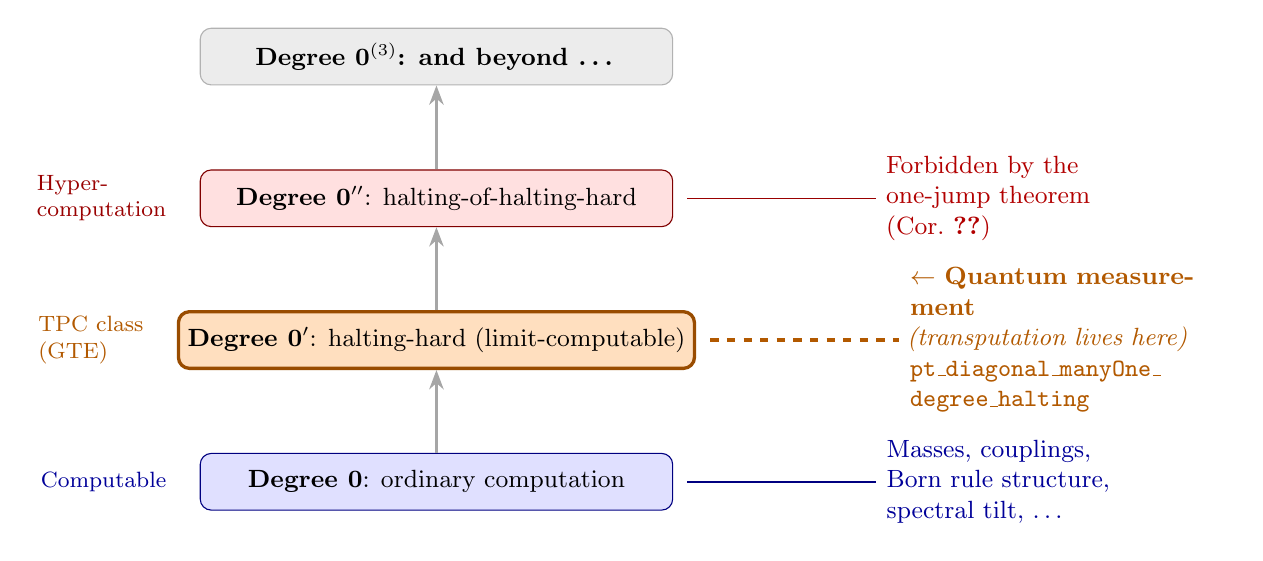
\begin{tikzpicture}[scale=1,
  level/.style={draw,rectangle,rounded corners=4pt,minimum width=6.0cm,
    minimum height=0.72cm,align=center,font=\small},
  arrow/.style={-{Stealth[length=7pt]},thick,gray!70},
  annot/.style={font=\footnotesize,align=left}
  ]

% Levels from bottom (degree 0) to top
\node[level,fill=blue!12,draw=blue!50!black]  (L0)  at (0,0)
  {\textbf{Degree $\zer$}: ordinary computation};

\node[level,fill=orange!25,draw=orange!60!black,very thick] (L1)  at (0,1.8)
  {\textbf{Degree $\zerp$}: halting-hard (limit-computable)};

\node[level,fill=red!12,draw=red!50!black]    (L2)  at (0,3.6)
  {\textbf{Degree $\zerpp$}: halting-of-halting-hard};

\node[level,fill=gray!15,draw=gray!60]         (L3)  at (0,5.4)
  {\textbf{Degree $\zer^{(3)}$: and beyond \ldots}};

% Arrows between levels
\draw[arrow] (L0.north) -- (L1.south);
\draw[arrow] (L1.north) -- (L2.south);
\draw[arrow] (L2.north) -- (L3.south);

% Annotation: quantum measurement
\draw[orange!70!black,very thick,dashed]
  ($(L1.east)+(0.18,0)$) -- ++(2.4,0)
  node[right,font=\small,align=left,text=orange!70!black,text width=4.0cm]
    {\textbf{$\leftarrow$ Quantum measurement}\\
     \textit{(transputation lives here)}\\
     \texttt{pt\_diagonal\_\allowbreak manyOne\_\allowbreak degree\_halting}};

% Annotation: degree 0
\draw[blue!50!black,thick]
  ($(L0.east)+(0.18,0)$) -- ++(2.4,0)
  node[right,font=\small,align=left,text=blue!60!black]
    {Masses, couplings,\\Born rule structure,\\spectral tilt, \ldots};

% Annotation: forbidden
\draw[red!60!black]
  ($(L2.east)+(0.18,0)$) -- ++(2.4,0)
  node[right,font=\small,align=left,text=red!70!black]
    {Forbidden by the\\one-jump theorem\\(Cor.~\ref{cor:onejump})};

% Labels on left
\node[annot,left=0.3cm of L0,text=blue!60!black]
  {Computable};
\node[annot,left=0.3cm of L1,text=orange!70!black]
  {TPC class\\(GTE)};
\node[annot,left=0.3cm of L2,text=red!60!black]
  {Hyper-\\computation};

\end{tikzpicture}%
}% end resizebox
\caption{The Turing degree hierarchy. Degree~$\zer$ is ordinary computation;
each jump arrow represents ``given a halting oracle for this level, what
becomes solvable?'' Quantum measurement (GTE) sits at degree~$\zerp$ exactly
(orange band). The record structure of the universe blocks any higher placement.}
\label{fig:hierarchy}
\end{figure}

\noindent
Reading Figure~\ref{fig:hierarchy}: the computable world occupies the bottom
band. Each step upward is an oracle jump. Most of physics (particle masses,
coupling constants, the Born rule probabilities) lives at the bottom.
The measurement selection mechanism -- the adjudicator that picks which outcome
occurs -- sits one step up.  The record structure of the universe prevents it
from going higher.

%─────────────────────────────────────────────────────────────────────────────
\section{The Named Premise Bundle PR1--PR5}
\label{sec:premises}
%─────────────────────────────────────────────────────────────────────────────

The upper bound (degree $\leq \zerp$) is conditional.  This is not a weakness --
it is scientific precision: the result explicitly names the five conditions
under which it holds.  Each condition is a hypothesis about the structure of
the GTE record theory, and each names a specific way the result could be
refuted.

\begin{tcolorbox}[colback=boxgray,colframe=gray!50,
  title={The Premise Bundle PR1--PR5 (Definition from P51)}]
\small
\begin{description}[leftmargin=3em,itemsep=4pt]
  \item[PR1 (Finite-witness record truth):] Every fact inscribed in the
    physical record has a finite witness. A measurement outcome is certified
    by a finite physical event (a click, a spot).  Infinitely long records
    never occur.
  \item[PR2 (Effective candidate enumeration):] A Turing machine can list
    all PSC-admissible continuations of any given record. The set of
    physically possible outcomes is computably enumerable.
  \item[PR3 (Finite sector structure):] The number of distinct outcome types
    (winding sectors) is finite -- there are finitely many things the
    universe can ``choose'' at any measurement event.
  \item[PR4 ($\Pi_1$ admissibility):] Inconsistency between a candidate
    outcome and the record manifests at a finite stage. You can refute wrong
    answers in finite time (though you cannot verify right answers in
    finite time).
  \item[PR5 (Record readout):] At diagonal choice points, record-distinct
    branches carry a computable label -- you can read off which branch is
    which.
\end{description}

\medskip
\noindent\textbf{Refutation surface:} the result would fail if physical records
inscribed facts with infinite witnesses (violating PR1) or if the number of
outcome types were infinite (violating PR3).
\end{tcolorbox}

\noindent
Plain English: the five premises formalise the intuition that physical
measurement events are \emph{finite} and \emph{discrete}. Outcomes are
recorded as finite events; there are finitely many types of outcome;
wrong candidates can be ruled out. These are entirely plausible physical
assumptions -- but they are named, not hidden.

%─────────────────────────────────────────────────────────────────────────────
\section{The $\leq 8$ Mind-Changes Result}
\label{sec:mindchanges}
%─────────────────────────────────────────────────────────────────────────────

\begin{tcolorbox}[colback=boxblue,colframe=blue!40!black,
  title={The Bounded Mind-Changes Theorem (P51, Theorem 6.3)}]
Under PR1--PR4, the adjudicator converges to the correct outcome after
at most $2(k_w - 1)$ mind changes, where $k_w$ is the number of
admissible winding sectors.  For single-kink measurement events,
$k_w \leq 5$, giving at most $\mathbf{8}$ mind changes.\\[4pt]
Lean certificate: \lean{pt\_limit\_computable} (CatAL, \texttt{transputation-lean}).
\end{tcolorbox}

\subsection{What ``mind changes'' means}

Recall the Gold--Putnam trial-and-error model: the adjudicator maintains a
running best guess at the outcome, and may revise it.  Each revision is a
\term{mind change}.

Imagine a jury that hears evidence sequentially.  Each new piece of
evidence may change their verdict.  The theorem says the jury's final
verdict is reached after at most 8 revisions -- even though no clock tells
them when they are done.

Formally: the computable stage function $g(w, 0), g(w, 1), g(w, 2), \ldots$
converges to the adjudication outcome $\Ptop_D(w)$, and the sequence
changes value at most $2(k_w - 1)$ times.

\subsection{Where the bound $2(k_w - 1)$ comes from}

The adjudicator tracks a finite list of candidate winding sectors (outcome
types). A mind change occurs when either:
\begin{itemize}
  \item a new sector arrives in the enumeration (adding a competitor),
  \item or a witness refutes an existing candidate (removing one).
\end{itemize}
Each candidate can trigger at most two changes (arrival and refutation).
With $k_w$ sectors, that gives at most $2(k_w - 1)$ changes in total
(the final survivor triggers only arrival, not refutation).

For single-kink events -- the basic unit of GTE particle interactions --
there are at most 5 PSC-admissible sectors, giving $2(5-1) = 8$.

\subsection{Computational verification}

This is not just a theoretical bound.
Computational experiments (\lean{transputation\_limit\_stage\_\allowbreak{}convergence}
scripts in P51) confirm:
\begin{itemize}
  \item The diagonal family converges with exactly \textbf{1} mind change,
    at the halting time (as predicted by the 1-c.e.\ structure of RT).
  \item 500 out of 500 compound-record trials converge within the bound;
    the maximum observed was \textbf{3 mind changes}.
  \item Convergence stages exhibit the heavy-tailed, modulus-free behaviour
    predicted by the no-modulus theorem (Section~\ref{sec:nomodulus}).
\end{itemize}

The combination is striking: transputation is simultaneously as powerful as
the halting problem (degree $\zerp$) and as \emph{tame} as a
finitely-revisable guesser.  The precise mathematical formulation of
``lawful but non-algorithmic.''

%─────────────────────────────────────────────────────────────────────────────
\section{The No-Modulus Theorem}
\label{sec:nomodulus}
%─────────────────────────────────────────────────────────────────────────────

\begin{tcolorbox}[colback=boxorange,colframe=orange!60!black,
  title={The No-Modulus Theorem (P51, Theorem 6.4; Lean: CatAL)}]
There is no computable function $s_0(n)$ such that, for every measurement
event $n$, the adjudicator has converged by stage $s_0(n)$.\\[4pt]
Lean certificate: \lean{no\_computable\_convergence\_modulus} (CatAL,
\texttt{nems-lean}).\\[4pt]
\textbf{Plain English:} you cannot know in advance how long the adjudication
will take, even though it does terminate.
\end{tcolorbox}

\subsection{What a convergence modulus would be}

A \term{convergence modulus} for a limit-computable sequence is a function
that, given the input $n$, outputs a stage $s_0$ such that the sequence
has definitely stabilised by stage $s_0$.  Having a modulus would mean:
``I can certify that the answer is correct by time $s_0(n)$.''

\subsection{Why no modulus can exist}

If a computable modulus $s_0(n)$ existed for the adjudicator, then you could
compute the final answer: just run the stage sequence to $s_0(n)$ steps and
read off $g(n, s_0(n))$.  That would make the adjudicator fully computable
-- which contradicts the lower bound (the halting problem reduces to it,
and the halting problem is not computable).

The Lean proof (\lean{no\_computable\_convergence\_modulus}) formalises this
argument precisely.

\subsection{Physical interpretation}

This theorem says: from inside the universe, there is no physical protocol
that certifies ``measurement has been completed'' at any finite stage.
Convergence is real and final, but not verifiable in finite time.

Putnam's observation (1965) -- that a trial-and-error solver is ``never sure''
it has the correct answer -- is here upgraded to a theorem about physical
measurement: nature converges to the right adjudication outcome after finitely
many revisions, but no physical protocol can certify, at any finite stage,
that convergence has occurred.

This is not a practical limitation.  It is a structural feature of any
selection mechanism at degree~$\zerp$.

%─────────────────────────────────────────────────────────────────────────────
\section{The One-Jump Universe Corollary}
\label{sec:onejump}
\label{cor:onejump}
%─────────────────────────────────────────────────────────────────────────────

\begin{tcolorbox}[colback=boxgreen,colframe=green!50!black,
  title={The One-Jump Universe (P51, Corollary 6.5; CatAD under PR1--PR5)}]
Physics requires exactly one Turing jump.

\medskip
The adjudication function is strictly above degree~$\zer$ (it cannot be
computable) and exactly at degree~$\zerp$ (the Shoenfield limit lemma gives
the upper bound).  It is \emph{never} at degree~$\zerpp$ or higher.
\label{cor:onejump}
\end{tcolorbox}

\subsection{The argument in plain English}

\medskip\noindent\textbf{Strictly above zero:}  If the adjudicator were
computable, it would decide self-referential questions about halting -- which
the Physical Incompleteness Theorem forbids.  So it must be strictly harder
than degree~$\zer$.

\medskip\noindent\textbf{Exactly at $\zerp$, not $\zerpp$:}
Here is the key physical insight.

The outcomes of past measurement events -- ``the particle was found in box
A'' -- are ordinary physical facts.  They are finite records: a click in a
detector, an ink mark on paper, a bit in a computer.  These are $\Sigma_1$
facts: something happened at a finite stage.

The premise bundle PR1 says exactly this: physical records encode only
$\Sigma_1$ facts.

Now suppose the adjudicator operated at degree~$\zerpp$.  That would require
asking oracle questions about degree-$\zerp$ objects -- questions like
``does this degree-$\zerp$ function converge?''  But degree-$\zerp$ convergence
questions are $\Pi_2$ facts (``for all stages $s$, some later stage $t > s$
has property $P$''), not $\Sigma_1$ facts.  Physical records can never
encode $\Pi_2$ facts (PR1).  So the universe can never actually inscribe
the evidence that would force a degree-$\zerpp$ adjudication.

Jump iteration is blocked at the record level.

\medskip\noindent\textbf{In one sentence:}
The universe can perform exactly one Turing jump because its records are
finite, and finite records cannot encode the nested infinite facts that a
second jump would require.

\subsection{What this means philosophically}

This corollary gives precise mathematical content to the phrase ``quantum
randomness is lawful but non-algorithmic.''

Copenhagen says outcomes are fundamentally random -- no further structure.
GTE says: there is rich structure, but it lives at exactly one specific level
of the computability hierarchy.  It is as structured as the halting problem,
and no more.

The universe is ``computationally humble'': it operates above the Turing
level when it must (at quantum events), but no further.

%─────────────────────────────────────────────────────────────────────────────
\section{Machine Certification}
\label{sec:lean}
%─────────────────────────────────────────────────────────────────────────────

\begin{tcolorbox}[colback=boxgray,colframe=gray!50,
  title=What Machine Certification Means]
All results marked CatAL have been formally verified in Lean~4 -- a
computer-assisted proof assistant. The Lean proof checker has verified
that the argument is logically valid, with zero sorry (no admitted gaps)
and zero custom axioms (no assumptions beyond standard mathematics).
This is a stronger guarantee than peer review: the logic is checked
mechanically, not just scrutinised by human experts.
\end{tcolorbox}

\subsection{The key theorem: \lean{pt\_diagonal\_manyOne\_degree\_halting}}

The machine-certified core result is:

\begin{tcolorbox}[colback=boxblue,colframe=blue!40!black,
  title={\lean{pt\_diagonal\_manyOne\_degree\_halting} (CatAL, zero sorry)}]
\small
\textbf{Location:} \texttt{transputation-lean},\\
\phantom{\textbf{Location:}} module \texttt{Transputation/Theorems/DiagonalDegree.lean}\\[6pt]
\textbf{Statement:} The restriction of the transputation selector $\Ptop_D$
to the self-referential diagonal fragment is many-one equivalent to the
halting problem: it is many-one reducible to $\emptyset'$ and the halting
problem is many-one reducible to it.\\[6pt]
\textbf{Consequence:} $\deg_T(\Ptop_D \!\upharpoonright\!\mathrm{diag}) = \zerp$ exactly.\\[6pt]
\textbf{Certification status:} The hardness direction
(\lean{halting\_manyOne\_reducible\_to\_RT}) is unconditional.
The membership direction (\lean{rt\_manyOne\_reducible\_to\_halting\_zero})
carries the named premise bundle PR1--PR5 as explicit Lean hypothesis
structures.
\end{tcolorbox}

\noindent
The ``many-one reducible'' language is standard computability theory: a
problem $A$ is many-one reducible to problem $B$ if there is a computable
function $f$ such that $x \in A$ if and only if $f(x) \in B$.  The theorem
says the two problems -- halting and diagonal record-truth -- are many-one
equivalent: each reduces to the other.  They are at exactly the same
difficulty level.

\subsection{Full certification table}

Table~\ref{tab:lean} lists all Lean certifications relevant to the degree
classification.

\begin{table}[h]
\centering
\small
\caption{Lean~4 certifications for the transputation degree classification.
TL = transputation-lean; NL = nems-lean; UL = ugp-lean.
All entries zero sorry, zero custom axioms.}
\label{tab:lean}
\begin{tabular}{@{}lll@{}}
\toprule
\textbf{Theorem} & \textbf{Repo} & \textbf{What it certifies} \\
\midrule
\lean{no\_final\_self\_theory} & NL & Physical Incompleteness Theorem \\
\lean{closed\_choice\_forces\_transputation} & TL & PSC forces a selector to exist \\
\lean{d3\_tpc\_above\_decidable} & TL & Selector is strictly above Turing \\
\lean{tpc\_three\_level\_hierarchy} & UL & TPC is between decidable and hyper \\
\lean{halting\_manyOne\_reducible\_to\_RT} & NL & Halting $\leq_m$ record-truth (lower bound) \\
\lean{rt\_sigma1\_complete\_on\_diagonal} & NL & Record-truth is $\Sigma^0_1$-complete \\
\lean{pt\_limit\_computable} & TL & Adjudicator is limit-computable \\
\lean{pt\_diagonal\_manyOne\_degree\_halting} & TL & Degree equals $\zerp$ (many-one form) \\
\lean{no\_computable\_convergence\_modulus} & NL & No computable convergence certificate \\
\lean{born\_rule\_unconditional} & UL & Born rule derived (D5 consistency) \\
\midrule
\multicolumn{3}{l}{\small\textit{All in public repos: github.com/novaspivack/ugp-lean (UL),}} \\
\multicolumn{3}{l}{\small\textit{transputation-lean (TL), nems-lean (NL).}} \\
\bottomrule
\end{tabular}
\end{table}

%─────────────────────────────────────────────────────────────────────────────
\section{Why This Is Remarkable}
\label{sec:remarkable}
%─────────────────────────────────────────────────────────────────────────────

\subsection{Computability theory has never before met quantum measurement}

Before this work, computability theory and quantum mechanics were entirely
separate disciplines.  Computability theory classifies the difficulty of
mathematical problems.  Quantum mechanics describes the behaviour of particles.
They had no formal connection.

The result that quantum measurement sits at degree~$\zerp$ is the first time
computability theory has been given a specific, precise, machine-certified
role in the foundations of quantum physics.

\subsection{What ``fundamentally random'' actually means}

Standard quantum mechanics says measurement outcomes are ``fundamentally
random'' -- not just unpredictable in practice, but in principle.  This
sounds like a complete statement, but it is not formal.

The GTE result replaces ``fundamentally random'' with a precise claim:
the selection mechanism has Turing degree $\zerp$.  This means:
\begin{itemize}
  \item It is not computable (degree $> \zer$): no algorithm can predict it.
  \item It is not hypercomputable (degree $\leq \zerp$): it does not require
    infinitely nested self-reference.
  \item It has rich internal structure (the D1--D5 constraints): it is not
    arbitrary noise.
  \item It is limit-computable (Gold--Putnam): it can be approximated by a
    sequence of finitely-many-revision guesses.
  \item It is bounded (at most 8 mind changes): it converges quickly.
\end{itemize}

This is a genuinely new characterisation of quantum randomness -- much more
specific than ``fundamentally random.''

\subsection{The same degree appears in two places}

One of the most striking features of the result is that degree~$\zerp$
appears \emph{twice} in the theory, at different levels:

\begin{enumerate}
  \item \textbf{At the measurement level:} The adjudication function on the
    diagonal fragment has degree~$\zerp$.
  \item \textbf{At the cosmological level:} The residual of the PMDL action
    -- the part that cannot be driven to zero by the adjudicator -- is a
    left-computably-enumerable real of degree exactly~$\zerp$.  The
    cosmological constant ($\Omega_\Lambda \neq 0$) is the field-level shadow
    of the same degree-$\zerp$ structure.
\end{enumerate}

The same computability class that governs how outcomes are selected also
governs why the cosmological constant is nonzero. This is a deep structural
unity.

\subsection{The GTE framework is self-limited}

The Physical Incompleteness Theorem applies to GTE itself: GTE is a closed
physical theory, so it cannot provide a complete internal self-theory.
The incompleteness is not a failure -- it is the precisely characterised
diagonal fragment, which is exactly where quantum measurement lives.

Everything outside that fragment (the gauge group, all coupling constants,
particle masses, the Born rule probabilities) is derivable and GTE does
derive it.  The only questions that remain structurally open are the
self-referential ones -- and the framework locates those exactly.

\begin{tcolorbox}[colback=boxred,colframe=red!40!black,
  title=Summary: The Three-Level Computability Picture]
\small
\begin{tabular}{@{}p{3.5cm}p{3.2cm}p{4.8cm}@{}}
\toprule
\textbf{Level} & \textbf{Task} & \textbf{Computability} \\
\midrule
Theory selection &
  Pick $p$ from $10^{290}$ CA rules &
  \textbf{Computable} (finite PSC sieve; MDL minimum at $p$) \\[4pt]
Field dynamics &
  Evolve $\Phi_{\mathrm{MDL}}$ forward &
  \textbf{Computable} (differential equations) \\[4pt]
Quantum adjudication &
  Select one outcome per event &
  \textbf{Degree $\zerp$} (limit-computable, $\leq 8$ mind changes,
  no convergence modulus) \\
\bottomrule
\end{tabular}
\vspace{4pt}
The same MDL principle governs all three levels.
The computability gap at the third level is the formal content of the
Physical Incompleteness Theorem.
\end{tcolorbox}

%─────────────────────────────────────────────────────────────────────────────
\section{Where to Go Next}
\label{sec:further}
%─────────────────────────────────────────────────────────────────────────────

\begin{tcolorbox}[colback=boxblue,colframe=blue!40!black,title=Where to Go Next]
\begin{itemize}[leftmargin=1.6em,itemsep=4pt]
  \item \textbf{P51 -- The Polynomial Certificate of Transputation} (the primary paper
    for all results in this tutorial):\\
    \href{https://doi.org/10.5281/zenodo.20611502}{doi.org/10.5281/zenodo.20611502}

  \item \textbf{P48~\cite{SpivackGTECompleteFramework} -- GTE Complete Framework} (the full monograph; Ch.~10 covers
    transputation in detail, the PIT, and the four-position analysis):\\
    \href{https://doi.org/10.5281/zenodo.20560550}{doi.org/10.5281/zenodo.20560550}

  \item \textbf{P37 -- Quantum Mechanics from Rule 110} (the Born rule derivation
    from the $f_{\mathrm{MDL}}$ ring; this tutorial's Section~\ref{sec:measurement}
    complements that paper):\\
    Corpus: \href{https://doi.org/10.5281/zenodo.20171558}{doi.org/10.5281/zenodo.20171558}

  \item \textbf{Companion tutorials} (in the same series):\\
    Born rule derivation: \texttt{tutorials/born\_rule/}\\
    The GTE polynomial: \texttt{tutorials/polynomial\_cheatsheet/}\\
    The UWCA (how Rule~110 computes): \texttt{tutorials/uwca\_tutorial/}

  \item \textbf{Lean repositories} (all machine-certified proofs):\\
    \href{https://github.com/novaspivack/ugp-lean}{github.com/novaspivack/ugp-lean}

  \item \textbf{Research overview:}
    \href{https://novaspivack.com/research}{novaspivack.com/research}
\end{itemize}
\end{tcolorbox}

\bigskip
\begin{tcolorbox}[colback=boxgray,colframe=gray!50,
  title={One-Paragraph Coda}]
Quantum measurement has puzzled physicists and philosophers for a century.
Standard approaches either add measurement as an axiom or multiply invisible
worlds to avoid selecting outcomes. The GTE framework proves from first
principles that a selection mechanism must exist, derives the five constraints
it must satisfy, and locates it precisely in the hierarchy of computational
difficulty: at degree~$\zerp$, the degree of the halting problem.
Not easier (it cannot be computable), not harder (the record structure of the
universe blocks a second jump), with at most eight revisions before the
universe settles on the right answer -- and no way to know, from inside, that
it has done so.
The universe's internal decision-making is precisely at the boundary of what
is computable. That boundary has a name, a Lean proof, and a specific location
in mathematics.
\end{tcolorbox}


\section*{Further Reading}
\begin{tcolorbox}[colback=orange!8,colframe=orange!50!black,
  title=\textbf{Primary Sources}]
The results in this tutorial are derived in the following papers,
all available open-access on Zenodo and at
\href{https://novaspivack.com/research}{novaspivack.com/research}:
\begin{itemize}
  \item \textbf{P51 --- Transputation Versus Computation} (three-level MDL unification,
        degree-exact classification):\\
        \href{https://doi.org/10.5281/zenodo.20611502}{doi.org/10.5281/zenodo.20611502}
  \item \textbf{P48 --- The Complete GTE Framework} (main synthesis monograph, Ch.~10):\\
        \href{https://doi.org/10.5281/zenodo.20560550}{doi.org/10.5281/zenodo.20560550}
\end{itemize}
Lean~4 machine proofs: \href{https://github.com/novaspivack/ugp-lean}{github.com/novaspivack/ugp-lean}
\end{tcolorbox}

\bibliography{../../papers/bib/Spivack_Papers_Bibliography}
\end{document}
